\chapter{Introduction}\label{sec:Introduction}
\pagenumbering{arabic}
\setcounter{page}{1}
As the technology evolves it unlocks more and more possibilities. Just few years back there were no smart watches or phones but at this time they are important part of our lives. As they evolve there is the need for them to have more functions and features. One of them is to locate it's position on the map. This information is very useful since it can prevent people from getting lost, figuring out path to drive, used by military and countless more cases.

Finding out such position is possible using Global Navigation Satellite System (GNSS). Multiple implementations of this system exist like GPS, GLONASS or Galileo. All of these systems provide location using sufficient number (at least 4) of satellites.\cite{GNSS} GNSS solution requires clear path between satellites and the receiving device because signal is not able to pass through buildings. That makes it the main reason why it cannot be used for indoor localization.

There are multiple approaches to find out location inside the building. They can be divided into three main types. First type is using wireless signal ranging approach with multiple kinds of data like Time of Arrival (ToA). Second approach is using special equipment like active bats (Ultrasonic). And final type based on Signal Strength Fingerprint Maps (SSFM), in which first part is to collect signal strengths from the environment and construct fingerprint maps. They are then used to match with current signal to obtain the location.\cite{LocalizationApproaches}

\begin{figure}[h!]
	\begin{centering}
		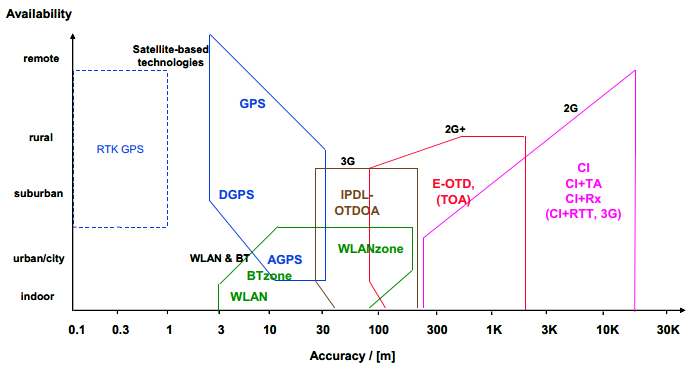
\includegraphics[width=0.7\textwidth]{img/1_comparison_of_positionin_technologies}
		\par\end{centering}
	\caption{Comparison of Positioning Technologies (source: \cite{PedestrianDeadReckoning})\label{fig:1_comparison_of_positionin_technologies}}
\end{figure}

In addition to these types there are also multiple algorithms used in indoor localization. Some of them are location fingerprinting, triangulation, proximity and dead reckoning.\cite{AaPLocalisation} Description of few algorithms can be found in chapter 2.

This thesis is focused on method using radio signal strength (RSS) fingerprinting collecting data from bluetooth, wireless and cellular networks.

\section{Goals of this thesis}\label{sec:GoalsOfThisThesis}
Main goal of this thesis is to explore possibilities of fingerprint collection using smart watch technology. The first question that needs to be answered is if this can be done. Is smart watch capable of RSS data collection? And the answer to this question is yes since smart watches have the similar specifications as low-end smart phones. 

One of the goals for this thesis is to create an application for Android phone and wear device which handles fingerprint collection. Problem with smart watches is their diversity in operational system because a lot of watch creators build their own custom systems which can complicate things. Luckily there is new system from Android called Wear 2.0 and it is basically port of Android system to wearable devices. 

And final goal is to test created application and figure out if it's data are useful for indoor localization or not.

\section{Reason for selection of this topic}\label{sec:ReasonForSelectionOfThisTopic}
The reason behind selection of this topic is rather simple. I was introduced to Android during my studies at the University but it was not any deep knowledge so I decided to go for a study abroad to deepen my knowledge. Part of that study was to work for a company where we developed rather technical heavy Android application. It's core part was using multiple APIs but it was focused only on a singe device. So next thing I wanted try was working with multiple kinds of devices and since Android Wear 2.0 is rather new I wanted to test it out. So the main reason is to get more experienced with Android and as a developer.